\documentclass[10pt]{amsart}
\usepackage{lmodern}

\makeatletter
\ifcase \@ptsize \relax% 10pt
  \newcommand{\miniscule}{\@setfontsize\miniscule{4}{5}}% \tiny: 5/6
\or% 11pt
  \newcommand{\miniscule}{\@setfontsize\miniscule{5}{6}}% \tiny: 6/7
\or% 12pt
  \newcommand{\miniscule}{\@setfontsize\miniscule{5}{6}}% \tiny: 6/7
\fi
\makeatother

\usepackage{changepage}
%     If your article includes graphics, uncomment this command.
\usepackage{colortbl}
%\usepackage{graphicx}
\usepackage{leftidx}
\usepackage{mathtools}
\usepackage{graphicx}

\usepackage{expl3}
\ExplSyntaxOn
\cs_new_eq:NN \fpeval \fp_eval:n
\cs_new_eq:NN \clistitem \clist_item:Nn
\cs_new_eq:NN \foreachint \int_step_inline:nnnn
\ExplSyntaxOff

\usepackage{pgf}
\usepackage{pgf-spectra}
%\usepackage{fp}
%\usetikzlibrary{fpu}
%\usetikzlibrary{fpu}

%\pgfkeys{/pgf/fpu=true}

\newcommand{\eq}{=}
\newcommand{\setvalue}[1]{\pgfkeys{/variables/#1}}
\newcommand{\getvalue}[1]{\pgfkeysvalueof{/variables/#1}}
\newcommand{\declare}[1]{%
 \pgfkeys{
  /variables/#1.is family,
  /variables/#1.unknown/.style = {\pgfkeyscurrentpath/\pgfkeyscurrentname/.initial = ##1}
 }%
}
\pgfkeys{/pgf/number format/.cd ,precision=12,sci generic={exponent={\times 10^{#1}}}}
%\pgfset{fpu=true}


\usepackage{gnuplottex}
\usepackage{siunitx}
%\usepackage{subcaption}
%\usepackage{subfigure}
\usepackage{float}
\newcommand{\sinc}{\operatorname{sinc}}
\newcommand{\rect}{\operatorname{rect}}
\newcommand{\wll}{\textcolor{white}{123}}
\newcommand{\tot}{\text{tot}}
\newcommand{\ptl}{\text{ptl}}
\newcommand{\ove}{\operatorname{vec}}
\newcommand{\apr}{\text{apparatus}}
\newcommand{\dtr}{\text{dtr}}
\newcommand{\initial}{\text{initial}}
\newcommand{\final}{\text{final}}
\newcommand{\BS}{\operatorname{BS}}
\newcommand{\path}{\text{path}}
\newcommand{\up}{\uparrow}
\newcommand{\down}{\downarrow}
%\usepackage[dvipsnames]{xcolor}

%\usepackage[x11names]{xcolor}
\newtagform{blue}{\color{blue}(}{)}
%\usepackage[dvipsnames]{xcolor}

%\usepackage{pgfplots} 
 %   \usetikzlibrary{intersections}
    % use this `compat' level or higher so that TikZ coordinates don't have to be prefixed
    % with `axis cs:'
  %  \pgfplotsset{width=15cm,compat=1.11}
\usepackage{amsthm}
\usepackage{amsmath,amssymb}
\usepackage{helvet}
%\usepackage[leqno]{amsmath}
%\usepackage{blindtext}
\usepackage{bbm}

\makeatletter
\newcommand{\newparallel}{\mathrel{\mathpalette\new@parallel\relax}}
\newcommand{\new@parallel}[2]{%
  \begingroup
  \sbox\z@{$#1T$}% get the height of an uppercase letter
  \resizebox{!}{\ht\z@}{\raisebox{\depth}{$\m@th#1/\mkern-5mu/$}}%
  \endgroup
}
\makeatother



\DeclareSymbolFont{extraup}{U}{zavm}{m}{n}
\DeclareMathSymbol{\varheart}{\mathalpha}{extraup}{86}
\DeclareMathSymbol{\vardiamond}{\mathalpha}{extraup}{87}
\newcommand{\redheart}{\textcolor{red}{$\varheart$}}
\newcommand{\heart}{\ensuremath\varheart}

%\definecolor{orange}{rgb}{1.0, 0.7, 0}
\definecolor{awesome}{rgb}{1.0, 0.13, 0.32}
\definecolor{}{rgb}{0.0, 0.0, 0.60}
\makeatletter\newcommand{\leqnomode}{\tagsleft@true\let\veqno\@@leqno}
\newcommand{\reqnomode}{\tagsleft@false\let\veqno\@@eqno}\makeatother

\makeatletter
\newcommand{\pushright}[1]{\ifmeasuring@#1\else\omit\hfill$\displaystyle#1$\fi\ignorespaces}
\newcommand{\pushleft}[1]{\ifmeasuring@#1\else\omit$\displaystyle#1$\hfill\fi\ignorespaces}
\makeatother

\makeatletter
\newcommand{\specialcell}[1]{\ifmeasuring@#1\else\omit$\displaystyle#1$\ignorespaces\fi}
\makeatother

%\newcommand{\subsec}[1]{\begin{adjustwidth}{-0.1in}{0in}\Large\textbf{\textcolor{darkblue}{#1}}\end{adjustwidth}\normalsize \vspace{1ex}}

\newcommand{\linebreakc}{\textcolor{white}{bl}\\}
\usepackage[english]{babel}
\usepackage[utf8]{inputenc}
% use KoTeX package for Korean 
\usepackage{kotex}
% for the fancy \koTeX logo
\usepackage{kotex-logo}


\newcommand{\expp}[1]{\exp\left(#1\right)}
\newcommand{\expb}[1]{\exp\left[#1\right]}
\newcommand{\sinb}[1]{\sin\left[#1\right]}
\newcommand{\cosb}[1]{\cos\left[#1\right]}
\newcommand{\sinp}[1]{\sin\left(#1\right)}
\newcommand{\cosp}[1]{\cos\left(#1\right)}

\newcommand{\logb}[1]{\log\left[#1\right]}
\newcommand{\lnb}[1]{\ln\left[#1\right]}
\newcommand{\logp}[1]{\log\left(#1\right)}
\newcommand{\lnp}[1]{\ln\left(#1\right)}


\usepackage{hyperref}
\usepackage[nameinlink,capitalize]{cleveref}
\hypersetup{
    colorlinks=true,
    linkcolor=blue,
    filecolor=magenta,      
    urlcolor=blue,
    pdftitle={PH475 Quantum Information I},
    bookmarks=true,
    pdfpagemode=FullScreen,
    }
\let\oldref\ref
\renewcommand{\ref}[1]{(\oldref{#1})} 
\def\equationautorefname~#1\null{(#1)\null}
\newcommand{\tagg}[1]{\stepcounter{equation}\tag{\theequation}\label{#1} }
\urlstyle{same}
\newcommand{\taggg}[1]{\tag{#1}\label{#1} }
%\usepackage{subfig}


%\numberwithin{equation}{section}

%\numberwithin{example}{section}
%\usepackage{subfig}

%\numberwithin{subfigure}{figure}

%\captionsetup[subfigure]{subrefformat=simple,labelformat=simple,listofformat=subsimple}
%\renewcommand\thesubfigure{(\alph{subfigure})}


\newtheorem{theorem}{Theorem}
\newtheorem*{theorem*}{Theorem}
\numberwithin{theorem}{section}

\newtheorem{lemma}{Lemma}
\newtheorem{proposition}{Proposition}

\newtheorem{exercise}{Exercise}
\newtheorem*{exercise*}{Exercise}
\crefname{exercise}{Exercise}{exercises}

\newtheorem{example}{Example}
\newtheorem*{example*}{Example}
\numberwithin{example}{section}
%\newtheorem{lemma}[lemma]{Lemma}
%\newtheorem{proposition}[theorem]{Proposition}
\newtheorem{corollary}[theorem]{Corollary}

%\newtheorem{exercise}[theorem]{Exercise}





\newtheorem{remark}[theorem]{Remark}
\newtheorem*{remark*}{Remark}
\newtheorem{problem}{Problem}
\newtheorem*{problem*}{Problem}

\newtheorem{innercustompro}{Problem}
\newenvironment{prob}[1]
  {\renewcommand\theinnercustompro{#1}\innercustompro}
  {\endinnercustompro}




\newtheorem{innercustomlem}{Lemma}
\newenvironment{lem}[1]
  {\renewcommand\theinnercustomlem{#1}\innercustomlem}
  {\endinnercustomlem}
  
\newtheorem{innercustomthm}{Theorem}
\newenvironment{thm}[1]
  {\renewcommand\theinnercustomthm{#1}\innercustomthm}
  {\endinnercustomthm}


\newenvironment{prf}
  {\begin{proof}[\textbf{\textcolor{magenta}{Proof}}\\]}
  {\end{proof}}
\makeatletter
  \renewcommand\@upn{\textit}
\makeatother



\newenvironment{solution}
  {\begin{proof}[\textbf{\textcolor{blue}{Solution}}\\]}
  {\end{proof}}
\makeatletter
  \renewcommand\@upn{\textit}
\makeatother

\newcommand{\lf}{\left}
\newcommand{\rg}{\right}
\theoremstyle{definition}
\newtheorem{definition}{Definition}
\newtheorem*{definition*}{Definition}

\newtheorem{innercustomdefi}{Definition}
\newenvironment{defi}[1]
  {\renewcommand\theinnercustomdefi{#1}\innercustomdefi}
  {\endinnercustomdefi}

%\newtheorem{example}{Example}

%\newtheorem{xca}[theorem]{Exercise}

\newtheorem{innercustomex}{Example}
\newenvironment{ex}[1]
  {\renewcommand\theinnercustomex{#1}\innercustomex}
  {\endinnercustomex}

\theoremstyle{remark}


%\newenvironment{proposition}[2][Proposition]{\begin{trivlist}
%\item[\hskip \labelsep {\bfseries #1}\hskip \labelsep {\bfseries #2.}]}{\end{trivlist}}


\newcommand{\abs}[1]{\left\lvert#1\right\rvert}

\definecolor{hotpink}{rgb}{1.0, 0, 0.6}
\definecolor{inter}{rgb}{0.4, 0.4, 1}
\definecolor{awesome}{rgb}{1.0, 0.13, 0.32}
\definecolor{darkblue}{rgb}{0.0, 0.0, 0.60}
\definecolor{darkgreen}{rgb}{0.0, 0.50, 0.0}
\definecolor{darkyellow}{rgb}{0.80, 0.80, 0.0}
\newcommand{\red}[1]{\textcolor{red}{#1}}
\newcommand{\rred}[1]{\textcolor{RubineRed}{#1}}
\newcommand{\dblue}[1]{\textcolor{darkblue}{#1}}
\newcommand{\dgreen}[1]{\textcolor{darkgreen}{#1}}
\newcommand{\blue}[1]{\textcolor{blue}{#1}}
\newcommand{\cyan}[1]{\textcolor{cyan}{#1}}
\newcommand{\magenta}[1]{\textcolor{magenta}{#1}}
\newcommand{\brown}[1]{\textcolor{brown}{#1}}
\newcommand{\dyellow}[1]{\textcolor{darkyellow}{#1}}
\newcommand{\am}[1]{\textcolor{Aquamarine}{#1}}

\newcommand{\purple}[1]{\textcolor{purple}{#1}}

\newcommand{\green}[1]{\textcolor{green}{#1}}
\newcommand{\orange}[1]{\textcolor{orange}{#1}}

\newcommand{\ot}{\otimes}
\newcommand{\rh}{\rho}
\newcommand{\tht}{\theta}
\usepackage{answers}
\usepackage{setspace}
\usepackage{graphicx}
\usepackage{enumerate}
\usepackage{multicol}
\usepackage{amssymb}
\usepackage{mathrsfs}
\usepackage[margin=1in]{geometry} 

\usepackage{braket}
\usepackage{CJKutf8}
\newcommand{\ob}[1]{\mkern 1.5mu\overline{\mkern-1.5mu#1\mkern-1.5mu}\mkern 1.5mu}
 
\newcommand{\N}{\mathbb{N}}
\newcommand{\iZ}{\mathbb{Z}}
\newcommand{\C}{\mathbb{C}}
\newcommand{\R}{\mathbb{R}}
\newcommand{\Q}{\mathbb{Q}}
\newcommand{\X}{\mathcal{X}}
\newcommand{\Y}{\mathcal{Y}}
\newcommand{\Z}{\mathbb{Z}}
\newcommand{\W}{\mathcal{W}}

\newcommand{\norm}[1]{\left\lVert#1\right\rVert}
\newcommand{\xra}[1]{\xrightarrow{#1}}
\newcommand{\E}{\mathbb{E}}
\newcommand{\V}{\operatorname{Var}} 
\newcommand {\tr} {\operatorname{Tr}}
\newcommand{\trp}[1]{\tr\left(#1\right)}
\newcommand{\trpp}[2]{\tr_{#1}\left(#2\right)}
\newcommand{\trb}[1]{\tr\left[#1\right]}

\newcommand*{\myfont}{\fontfamily{lmss}\selectfont}
\DeclareTextFontCommand{\fo}{\myfont}

%\usepackage{titlesec}

\makeatletter
%default definition of article.cls
%using \renewcommand instead of \newcommand
\renewcommand\part{%
   \if@noskipsec \leavevmode \fi
   \par
   \addvspace{4ex}%
   \@afterindentfalse
   \secdef\@part\@spart}

\def\@part[#1]#2{%
    \ifnum \c@secnumdepth >\m@ne
      \refstepcounter{part}%
      \addcontentsline{toc}{part}{\thepart\hspace{1em}#1}%
    \else
      \addcontentsline{toc}{part}{#1}%
    \fi
    {\parindent \z@ \raggedright
     \interlinepenalty \@M
     \normalfont
     \ifnum \c@secnumdepth >\m@ne
       \Large\bfseries \partname\nobreakspace\thepart
       \par\nobreak
     \fi
     \huge \bfseries #2%
     %%%\markboth{}{}\par}% removing redefinition of headings
     \par}%
    \nobreak
    \vskip 3ex
    \@afterheading}
\def\@spart#1{%
    {\parindent \z@ \raggedright
     \interlinepenalty \@M
     \normalfont
     \huge \bfseries #1\par}%
     \nobreak
     \vskip 3ex
     \@afterheading}
\makeatother

%\renewcommand{\partname}{Chapter}
%\newcommand{\part}{\part}
%\begin{comment}
%\titleformat{\part}
 % {\normalfont\myfont\huge\bfseries}
  %{\parttitlename\ \thepart}{20pt}{\huge}
%\end{comment}
  
  
\usepackage{etoolbox}
\patchcmd{\section}{\scshape}{\bfseries}{}{}
\makeatletter
\renewcommand{\@secnumfont}{\bfseries}
\makeatother  
  
%\renewcommand{\thesection}{\arabic{section}}  



\makeatletter
\def\@seccntformat#1{%
  \expandafter\ifx\csname c@#1\endcsname\c@section
  \thesection\hspace{2ex}
  \else
  \csname the#1\endcsname\quad
  \fi}
\makeatother

  
\makeatletter  
\renewcommand\partname{Chapter}
\renewcommand\part{\@startsection{part}{0}%
\z@{\linespacing\@plus\linespacing}{1\linespacing}%
{\myfont\bfseries\huge\raggedright}}  
\makeatother  
  
  

% http://joshua.smcvt.edu/latex2e/bs-at-startsection.html  
  
\makeatletter
\renewcommand\section{\@startsection{section}{1}%
{0pt}{.8\linespacing\@plus\linespacing}{.6\linespacing}%
{\LARGE\bfseries\color{black}}}
\makeatother

\makeatletter
\renewcommand\specialsection{\@startsection{specialsection}{1}%
{0pt}{.8\linespacing\@plus\linespacing}{.6\linespacing}%
{\LARGE\bfseries\color{hotpink}}}
\makeatother

\makeatletter
\renewcommand\subsection{\@startsection{subsection}{2}%
{0pt}{.8\linespacing\@plus.9\linespacing}{.7\linespacing}%
{\Large\bfseries\color{black}}}
\makeatother

\makeatletter
\renewcommand\subsubsection{\@startsection{subsubsection}{3}%
\z@{.6\linespacing\@plus.7\linespacing}{.4\linespacing}%
{\large\bfseries\color{black}}}
\makeatother

%https://tex.stackexchange.com/questions/268706/amsart-change-subsection-headings-from-boldface-to-smallcaps
%https://tex.stackexchange.com/questions/60437/newlines-after-section-headings-in-amsart
%http://ftp.ktug.org/tex-archive/macros/latex/required/amscls/doc/amsclass.pdf 의 Line 1175

\newcommand{\subsec}[1]{\begin{adjustwidth}{-0.1in}{0in}\subsection{#1}\end{adjustwidth}}
\newcommand{\subsect}[1]{\hspace{-0.2in}\subsection{#1}}
\newcommand{\secc}[1]{\begin{adjustwidth}{-0.1in}{0in}\section{#1}\end{adjustwidth}}

\usepackage{array}
\preto\tabular{\setcounter{magicrownumbers}{0}}
\newcounter{magicrownumbers}
\newcommand\rownumber{\small\stepcounter{magicrownumbers}\arabic{magicrownumbers}}


\newcommand{\vb}{\vec{B}}
\newcommand{\vj}{\vec{j}}
\newcommand{\vn}{\vec{\nabla}}
\newcommand{\vr}{\mathbf{r}}
\newcommand{\vk}{\mathbf{k}}
\newcommand{\va}{\vec{A}}
\newcommand{\vl}{\vect{l}}
\newcommand{\vp}{\varphi}\newcommand{\hvp}{\hat{\varphi}}
\setcounter{section}{+0}

\newcommand{\hq}{\hat{Q}}
\newcommand{\hp}{\hat{\Phi}}

\newcommand{\ha}{\hat{a}}
\newcommand{\hN}{\hat{N}}
\newcommand{\ld}{\lambda}
\newcommand{\htp}{\hat{p}}

\newcommand{\om}{\omega}
\newcommand{\var}{\operatorname{Var}}
\newcommand{\vect}{\mathbf}
\newcommand{\nul}{\operatorname{Nul}}
\newcommand{\col}{\operatorname{Col}}
\newcommand{\row}{\operatorname{Row}}
\newcommand{\dg}{\dagger}
%    Blank box placeholder for figures (to avoid requiring any
%    particular graphics capabilities for printing this document).
\newcommand{\blankbox}[2]{%
  \parbox{\columnwidth}{\centering
%    Set fboxsep to 0 so that the actual size of the box will match the
%    given measurements more closely.
    \setlength{\fboxsep}{0pt}%
    \fbox{\raisebox{0pt}[#2]{\hspace{#1}}}%
  }%
}



\usepackage{bbm}
%     If your article inludes graphics, uncomment this command
\usepackage{svg}
\usepackage[super, square]{natbib}
%\usepackage[square]{natbib}

%\usepackage{biblatex}
%\bibliography{name.bib}
\svgsetup{inkscapelatex=false}
\usepackage{epstopdf}
\usepackage{url}
%\usepackage{circuitikz}

\usepackage{pgf}
\usepackage{graphicx}
\usepackage{pgfplots}

\usepackage{gnuplottex}
\usepackage{pgfplotstable}
\usepgfplotslibrary{external} 
\usetikzlibrary{external}
%\tikzexternalize[prefix=tikz/]


%\pgfplotsset{every axis/.append style={
                    %axis x line=middle,    % put the x axis in the middle
                    %axis y line=middle,    % put the y axis in the middle
                    %axis line style={<->,color=blue}, % arrows on the axis
                    %xlabel={$x$},          % default put x on x-axis
                    %ylabel={$y$},          % default put y on y-axis
            %}}
\pgfplotsset{every tick label/.append style={font=\tiny}}
\pgfplotsset{every x tick label/.append style={font=\tiny, yshift=0.5ex}}
\pgfplotsset{every y tick label/.append style={font=\tiny, xshift=0.5ex}}
\pgfplotsset{ /pgf/number format/precision=10}

\begin{comment}

\pgfplotsset{
    node near coord/.style={ % Style for activating the label for a single coordinate
        nodes near coords*={
            \ifnum\coordindex=#1\pgfmathprintnumber{\pgfplotspointmeta}\fi
        }
    },
    nodes near some coords/.style={ % Style for activating the label for a list of coordinates
        scatter/@pre marker code/.code={},% Reset the default scatter style, so we don't get coloured markers
        scatter/@post marker code/.code={},% 
        node near coord/.list={#1} % Run "node near coord" once for every element in the list
    }
}

\pgfplotsset{
    node near coord/.style={ % Style for activating the label for a single coordinate
        nodes near coords*={
            \ifnum\coordindex=#1\pgfmathprintnumber{\pgfplotspointmeta}\fi
        }
    },
    nodes near some coords/.style={ % Style for activating the label for a list of coordinates
        scatter/@pre marker code/.code={},% Reset the default scatter style, so we don't get coloured markers
        scatter/@post marker code/.code={},% 
        node near coord/.list={#1} % Run "node near coord" once for every element in the list
    }
}

\pgfplotsset{
    node near coord/.style args={#1/#2/#3}{% Style for activating the label for a single coordinate
        nodes near coords*={
            \ifnum\coordindex=#1 #2\fi
        },
        scatter/@pre marker code/.append code={
            \ifnum\coordindex=#1 \pgfplotsset{every node near coord/.append style=#3}\fi
        }
    },
    nodes near some coords/.style={ % Style for activating the label for a list of coordinates
        scatter/@pre marker code/.code={},% Reset the default scatter style, so we don't get coloured markers
        scatter/@post marker code/.code={},% 
        node near coord/.list={#1} % Run "node near coord" once for every element in the list
    }

}

\pgfplotsset{
    node near coord/.style args={#1/#2/#3}{% Style for activating the label for a single coordinate
        nodes near coords*={
            \ifnum\coordindex=#1  #2\fi
        },
        scatter/@pre marker code/.append code={
            \ifnum\coordindex=#1 \pgfplotsset{every node near coord/.append style=#3}\fi
        }
    },
    nodes near some coords/.style={ % Style for activating the label for a list of coordinates
        scatter/@pre marker code/.code={},% Reset the default scatter style, so we don't get coloured markers
        scatter/@post marker code/.code={},% 
        node near coord/.list={#1} % Run "node near coord" once for every element in the list
    }

}

\end{comment}





\pgfplotsset{
    node near coord/.style args={#1/#2/#3}{% Style for activating the label for a single coordinate
        nodes near coords*={
            \ifnum\coordindex=#1\pgfmathprintnumber{\pgfplotspointmeta}#2\fi
        },
        scatter/@pre marker code/.append code={
            \ifnum\coordindex=#1 \pgfplotsset{every node near coord/.append style=#3}\fi
        }
    },
    nodes near some coords/.style={ % Style for activating the label for a list of coordinates
        scatter/@pre marker code/.code={},% Reset the default scatter style, so we don't get coloured markers
        scatter/@post marker code/.code={},% 
        node near coord/.list={#1} % Run "node near coord" once for every element in the list
    }
}


\pgfplotsset{
    pin near coord/.style args={#1/#2/#3}{% Style for activating the label for a single coordinate
        scatter/@pre marker code/.append code={
           \ifnum 1=#3
            \ifnum\coordindex=#1  point meta=x, \node[pin={#2:\small\color{black} \SI{\small\pgfmathprintnumber{\pgfplotspointmeta}}{\volt}  }]{};\fi 
            \fi 
            \ifnum 2=#3
            \ifnum\coordindex=#1 point meta=x, \node[pin={[align=center]75:#2}]{};\fi
            \fi
        }
    },
    pins near some coords/.style={ % Style for activating the label for a list of coordinates
        scatter,
        scatter/@pre marker code/.code={},% Reset the default scatter style, so we don't get coloured markers
        scatter/@post marker code/.code={},% 
        pin near coord/.list={#1} % Run "pin near coord" once for every element in the list
    }
}
\pgfplotsset{select coords between index/.style 2 args={
    x filter/.code={
        \ifnum\coordindex<#1\def\pgfmathresult{}\fi
        \ifnum\coordindex>#2\def\pgfmathresult{}\fi
    }
}}
%\usetikzlibrary {math, fpu}
%\pgfkeys{/pgf/fpu = true}
\usepackage{csvsimple}
\usepackage{ifpdf}
\usepackage{sidecap}
\usepackage{float}
\usepackage[labelformat=simple]{subcaption}
\renewcommand{\thesubfigure}{(\scshape\Alph{subfigure})}
\captionsetup[subfigure]{position=top}
\begin{comment}
\usepackage[labelformat=simple]{subcaption}
\renewcommand\thesubfigure{(\alph{subfigure})}
(Note: Since parens is the default label format you will get double parentheses in sub-captions if you don't specify a different label format, e.g., simple.)
\end{comment}
%\renewcommand\thesubfigure{(\alph{subfigure})}
\newcommand{\squeezeup}{\vspace{-5mm}}
\newcommand{\squeezeupp}{\vspace{-8.5mm}}
\newcommand{\squeezeuppp}{\vspace{-10mm}}
%\usepackage{pgfplots}
   % \usetikzlibrary{intersections}
    % use this `compat' level or higher so that TikZ coordinates don't have to be prefixed
    % with `axis cs:'
   %\pgfplotsset{width=15cm,compat=1.11}

\usepackage{siunitx}\sisetup{parse-numbers=false}
\sisetup{parse-numbers=false}
\DeclareSIUnit\torr{torr}
\DeclareSIUnit\gauss{G}
\usepackage{amsmath}
\usepackage{amsthm,amssymb}

\makeatletter
\def\convertto#1#2{\strip@pt\dimexpr #2*65536/\number\dimexpr 1#1}
\makeatother

% \usepackage{mhchem}
\usepackage{chemformula}
\let\ce\ch
\usepackage{longtable}
\usepackage{multirow, makecell}
\usepackage{multicol}
\begin{comment}

\makeatletter
\renewenvironment{thebibliography}[1]
     {\begin{multicols}{2}[\section*{\refname}]%
      \@mkboth{\MakeUppercase\refname}{\MakeUppercase\refname}%
      \list{\@biblabel{\@arabic\c@enumiv}}%
           {\settowidth\labelwidth{\@biblabel{#1}}%
            \leftmargin\labelwidth
            \advance\leftmargin\labelsep
            \@openbib@code
            \usecounter{enumiv}%
            \let\p@enumiv\@empty
            \renewcommand\theenumiv{\@arabic\c@enumiv}}%
      \sloppy
      \clubpenalty4000
      \@clubpenalty \clubpenalty
      \widowpenalty4000%
      \sfcode`\.\@m}
     {\def\@noitemerr
       {\@latex@warning{Empty `thebibliography' environment}}%
      \endlist\end{multicols}}
\makeatother
%\url{tex.stackexchange.com/questions/20758/bibliography-in-two-columns-section-title-in-one/20761}
\end{comment}
%\renewcommand{\bibpreamble}{\begin{multicols}{2}}
%\renewcommand{\bibpostamble}{\end{multicols}}
\usepackage{helvet}

\usepackage{blindtext}
\usepackage{mathtools}
%\usepackage[x11names]{xcolor}
%\newtagform{blue}{\color{blue}(}{)}
%\usepackage[dvipsnames]{xcolor}

\definecolor{awesome}{rgb}{1.0, 0.13, 0.32}
\definecolor{darkblue}{rgb}{0.0, 0.0, 0.60} 


\newcommand{\re}{\operatorname{Re}}
%\newcommand{\im}{\operatorname{Im}}
\newcommand{\im}{\implies}

%\newcommand{\redheart}{\textcolor{red}{$\varheartsuit$}}
%\newcommand{\heart}{\ensuremath\varheartsuit}



\usepackage[english]{babel}
\usepackage[utf8]{inputenc}
% use KoTeX package for Korean 
\usepackage{kotex}






%\numberwithin{equation}{section}

\usepackage{answers}
\usepackage{setspace}

\usepackage{enumerate}
\usepackage{enumitem}
\usepackage{multicol}
\usepackage{mathrsfs}
\usepackage[margin=1in]{geometry} 
\usepackage{changepage}
\usepackage{braket}
\usepackage{CJKutf8}


\DeclareTextFontCommand{\fo}{\myfont}

\newcommand*{\helve}{\fontfamily{phv}\selectfont}
\DeclareTextFontCommand{\fohe}{\helve}

\makeatletter
\newcommand*{\rom}[1]{\expandafter\@slowromancap\romannumeral #1@}
\makeatother


\begin{comment}
\newcommand{\vb}{\vec{B}}
\newcommand{\vj}{\vec{j}}
\newcommand{\vn}{\vec{\nabla}}
\newcommand{\vr}{\mathbf{r}}
\newcommand{\vk}{\mathbf{k}}
\newcommand{\va}{\vec{A}}
\newcommand{\vl}{\vect{l}}
\newcommand{\vp}{\varphi}\newcommand{\hvp}{\hat{\varphi}}
\setcounter{section}{+11}

\newcommand{\hq}{\hat{Q}}
\newcommand{\hp}{\hat{\Phi}}

\newcommand{\ha}{\hat{a}}
\newcommand{\hN}{\hat{N}}
\newcommand{\ld}{\lambda}
\newcommand{\htp}{\hat{p}}
%\usepackage[T1]{fontenc}
%\usepackage{bold-extra}
\newcommand{\var}{\operatorname{Var}}
\newcommand{\vect}{\mathbf}
\newcommand{\nul}{\operatorname{Nul}}
\newcommand{\col}{\operatorname{Col}}
\newcommand{\row}{\operatorname{Row}}
\newcommand{\dg}{\dagger}
\end{comment}
\usepackage{fancyhdr}
\usepackage{regexpatch}

\begin{comment}
%%% let's patch the amsart macros
\makeatletter
\renewcommand{\sectionmark}[2]{%
  \ifnum#1<\@m
    \markboth{\thesection. #2}{\thesection. #2}%
  \else
    \markboth{#2}{#2}%
  \fi}
\xpatchcmd*{\@sect}
  {\@tocwrite}
  {\csname #1mark\endcsname{#2}{#7}\@tocwrite}
  {}{}
\makeatother
\end{comment}

\pagestyle{fancy}
\fancyhf{}
%\rhead{}
\lhead{ }
%\fancyhead[L]{\rightmark}
\fancyhead[R]{\textcolor{black}{\thepage}}

%\renewcommand{\subsectionmark}[1]{%
%  \markright{\MakeUppercase{\thesubsection.\ #1}}}%

%\renewcommand{\sectionmark}[1]{%
%\markboth{\thesection\quad #1}{}}
%\fancyhead{}
%\fancyfoot[L]{\leftmark}
%\fancyfoot{}
%\fancyfoot[CE,CO]{\leftmark}
\cfoot{\thepage}
\newlength\FHoffset
\setlength\FHoffset{0.12in}

\addtolength\headwidth{2\FHoffset}

\fancyheadoffset{\FHoffset}

\usepackage{layouts}
\begin{document}
%\pgfset{fpu = true}
\usetagform{blue} \reqnomode
\newgeometry{left=0.9in, right=0.9in, top=1in, bottom=1in}
%\newgeometry{left=0.7in, right=0.7in, top=1in, bottom=1in}
\fancypagestyle{plain}{
  \fancyhf{}
  \lhead{ }
  \chead{}
  \rhead{\textcolor{black}{\thepage}}
}

\begin{center}
\linebreakc
\linebreakc
\linebreakc
\huge
%\textbf{\fo{ EXP 1.}}

\textbf{Anatomy Summary}

\textcolor{white}{bl}\\

\Large

Gyunghee Han

\end{center}

\textcolor{white}{bl}\\

\normalsize




\section{ Lumbar Plexus}
Lumbar plexus : L1, L2, L3, L4의 \textit{ \textbf{anterior rami}} 에서 유래 
\begin{enumerate}
\item 
iliohypogastric, ilioinguinal

L1 의 가지 
\item 
genitofemoral n, 


L1, L2 의 뿌리 2개가 합쳐져 만들어짐 


음부가지 
: deep inguinal ring을 통과해 
cremaster m.에 분포 

넓다리가지 
: iliacus m. 엉덩근을 가로질라 

고샅인대 inguinal ligament 뒤를 지나 thigh로 내려가 thigh \textbf{위안쪽 피부}신경이 됨 

\item lateral cutaneous nerve of thigh 

\textbf{가}쪽 \textbf{넙}다리 피부 신경은 

L2, L3에서 나옴 

\textbf{ㄱㄴ} \textit{\textbf{ㄷㅅ}} 
    \item femoral n. 
    
    : lumbar plexus의 가장 큰 신경
    
    L2, L3, L4의 anterior rami 
    
    \item  obturator n .
    
    L2, L3, L4의 anterior rami 
    
    \textbf{온엉덩혈관 뒤}\textit{}쪽 아래로 내려가 골반에 분포 
\end{enumerate}

\section{Abdominal Aorta의 가지 }
abdominal : diaphragm 밑 

$\implies $ 1st 가지가 inferior phrenic

\vspace{2pt}

\begin{enumerate}
\item inferior phrenic

\vspace{1.5pt}

\item suprarenal (superior, middle, inferior) 
\begin{enumerate}
    \item superior suprarenal ($\impliedby$ inferior phrenic)
    \item middle superarenal ($\impliedby$ abdominal aorta)
    
    middle : 그냥중간 : 가지가 아니라 그냥 aorta
    \item inferior suprarenal ($\impliedby $ renal a.)
    
    (inferior랑 supra 상쇄해서 없어져서 그냥 renal 됨) 
    
    
\end{enumerate}

\vspace{1.5pt}

    \item 
    celiac trunk 
    (복강동맥)
    
    \vspace{1.5pt}
    
    
    \item 
    
    Renal artery (LV 1$\sim$2) disc
    
    \vspace{1.5pt}
    
    
    \item 
    superior mesenteric a.
    
\end{enumerate}

\vspace{2pt}

\section{Inferior Vena Cava}
\begin{enumerate}
    \item 
    renal vein
    
    왼쪽이 더 길며 aorta 앞, superior mesenteric a. 뒤 
    
    \item 
    testicular vein, ovarian vein 
    : 왼쪽에서는 renal vein 으로 들어가고 
    
    오른쪽에서는 직접 ivc로 들어감 
\end{enumerate}

%----------------------------------------
\newpage
\section{Ureter 요관}

\subsection{길이와  위치 25}
25 cm \textbf{근육관}

LV 2$\sim$5의  Transverse process를 따라서 내려간다


Primary Retroperitoneal (Kidney와 마찬가지로 복막 뒤에 위치)

온엉덩동맥분기부를 가로질러 골반가장자리로  넘어간다. 


남성에서 정관은 복막의 요관주름(ureteric fold) 안 에서 요관과 교차한다.

남성에서 요관과 복막 사이를 지나가는 것은 정관 ((ductus deferens) 뿐이다.
(앞 -- 복막 -- 정관 -- 요관) 

여성에서 요관은 자궁동맥의 기원부위 안쪽으로 주행하여 자궁동맥이 요관 위를 가로지른다 .

water under bridge

요관의 아래끝은 방광정맥얼기가 둘러싼다. 

요관은 방광의 근육벽을 비스듬하게 아래안쪽으로 관통한다.

\subsection{좁은 부위 3개 - ureteral stone }

\begin{enumerate}
    \item pelvis와 요관의 경계 
    
    요관깔때기 연결부 
    (2mm)
    
    \item  
    요관이 엉덩혈관을 가로지르는 부분 (4mm)
    
    (동맥이 펄스가 세기 떄문에)
    
    \item 
    요관이 방광벽으로 들어가는 부분 (1mm) 
    가장좁다 
    
    
\end{enumerate}
요관결석은 요관에서 생성 (X)

콩팥의 pelvis에서 만들어진다. 


\subsection{Vein}

vesical venous plexus 
방광정맥얼기 $\xra{ \quad }$
inferior vesical vein 
$\xra{ \quad }$ internal iliac vein

\subsection{Artery}


\begin{enumerate}
    \item 배 
    
    성온배 
    \begin{enumerate}
        \item
        gonadal a.
        
        (testicular, ovarian )
        \item 
        common iliac 
        
        \item 
        abdominal 
    \end{enumerate}
    \item 골반 
    
    \begin{enumerate}
        \item 
        superior vesical 
        
        \item 
        internal iliac 
        \item  3,4,5,6 :  
        i u v m 
        
    \end{enumerate}
\end{enumerate}
\section{Kidney}

앞 (정동신)


\newpage
\section{Suprarenal Gland}


\textit{\textbf{perirenal fat capsule}}에 의해 둘러싸이고 \textit{\textbf{renal fascia}} 에 둘러싸여 diaphragm에 붙음

\textbf{\textit{renal capsule}}은 말 그대로 콩팥을 싸는 근막이므로 부신은 싸고있지 \textit{\textbf{않다}}. 



오른쪽 : triangular : 간이 오른쪽에 있어서 눌려서 세모 모양 

왼쪽 : semilunar

cortex : mesodermal,  medulla : ectodernal 외배엽 

\subsection{Arteries}

내분비기관이므로 혈관이 많은 가지를 쳐서 분포 

\begin{enumerate}
    \item superior suprarenal 
    $\impliedby$ inferior phrenic 
    
    \item middle suprarenal 
    $\impliedby$ abdominal aorta 
    
    \item inferior suprarenal 
    $\impliedby$ renal a. 
    
\end{enumerate}
이런 혈관들이 하나씩이 아니라 여러가지로 나온다 .

\subsection{Veins}


(recall : renal v.의 왼쪽이 더 긺)

\begin{itemize}
    \item left suprarenal v : left renal v. 로 들어감 
    
    \item 
    right suprarenal v. 
    : 직접 ivc 로 들어감 
    
\end{itemize}

(recall : renal v.의 왼쪽이 더 긺, 
오른쪽  renal v.는 짧아서 ivc로 직접들어간다 외우기 )

(혹은 ivc가 오른쪽으로 치우쳐있으므로  right는 직접 ivc로 left는 renal v.로 들어간다외우기)

(왼쪽 : 경우에따라 inf. phrenic v.로 들어가기도)

\newpage






\section{Diaphragm}
thoracic cavity와 abdominal cavity의 경계 

주변이 origin (이는 곳) : muscular part

중심이 insertion (닿는 곳) : central tendon

\begin{enumerate}
    \item 
    \textit{\textbf{sternal}} part
    \textit{\item \textbf{costal}} part
    \textit{\item \textbf{lumbar}} part 
    
    \begin{enumerate}
        \item median arcuate lig.
    
    right crus left crus 사이 대동맥이 지남     
        \item medial arcuate lig.
    
    psoas major m. 근막이 두꺼워진 것     
        \item lateral arcuate lig.
        
        qudrate lumborum m.의 근막이 두꺼워진 것 
        
        \item right crus 
        
        : 왼다리에 비해 크고 길다. 
        
        : 위쪽 3$\sim$4 개 허리뼈에서 시작된다. 
        
        (마지막 12째 갈비뼈 밑에,   허리뼈 위쪽에서 시작)
        
        \item left crus 
        
        :  위쪽 3개 허리뼈에서 시작된다. 
    \end{enumerate}
    
    \item sternocostal triangle 
    \item lumbocostal triangle
\end{enumerate}

 \subsection{Caval opening  (8th TV, 앞)}

in \textit{\textbf{central}} tendon 

\textit{\textbf{right}} side $\implies$  terminal branch of right phrenic n. 

right side인 이유 : \textit{\textbf{ivc가 오른쪽}}으로 치우쳐있으므로 

(right phrenic 전체가 caval opening 통과하는 것은 아님.

일부는 가로막 위에 분포, 일부는 caval opening통과하여 아래에 분포)


 숨을 들이쉬면
 
 \begin{enumerate}
     \item 
가로막이 수축하여 caval opening이 넓어짐  (origin인 주변쪽으로 수축하므로) $\implies$ ivc가 넓어짐 

\item  
 음압이 걸림 (공간이 넓어지므로)
 \end{enumerate}
(1), (2) $\implies$ 숨을 들이쉴 떄  심장으로 ivc의 정맥혈이 더 잘 돌아감 
\subsection{Esophageal Hiatus (10th TV, 중간)}

\textit{\textbf{right}} crus 사이 

\textit{\textbf{left}} gastric vessels의 esophageal branch,

vagus nn. ( \small{The branches of the right vagus nerve forms the posterior gastric plexus on the postero-inferior surface of the stomach, while the branches of the left vagus nerve forms the anterior gastric plexus on the antero-sup erior surface of the stomach.})


caval과 달리 tendon이 아니라 근육의 힘살 사이므로  근육이 수축하면 구멍이 좁아짐 $\implies$ 식도의 조임근 역할 
\subsection{Aortic Hiatus (12th TV, 뒤)}

\textit{\textbf{thoracic}} duct,  \textit{\textbf{azygos}} vein 

뒤는 diaphragm이 아니라 vertebra : 엄밀히는 diaphragm의 뒤 

\subsection{SternoCostal Triangle}
lymphatics

superior epigastric artery and vein  ( from  internal thoracic a.)

\subsection{뒤쪽의 작은 틈새 구멍들 }

sympathetic trunks 

splanchnic nerves 


\subsection{Artery}
\begin{enumerate}
    \item 
    PericardiaCo phrenic 
    a. (쭉 내려가는 $\impliedby$ internal thoracic)
    
 
    \item  Musculophrenic  (돌아가는) ($\impliedby$ internal thoracic)
    
    \item superior phrenic a. ($\impliedby$ descending thoracic aorta에서 직접 나옴)
    
    \item inferior phrenic a. ($\impliedby$ abdominal aorta TV12)
    
    
\end{enumerate}
(1), (2), (3)은 가슴 안의 동맥 

\noindent (4)는 배의 동맥


   \begin{remark}
        internal thoracic 
        
        \begin{enumerate}
            \item 
            pericardiaCophrenic (가로막 위)
            \item musculophrenic (가로막 위) (internal thoracic의 종말가지 1)
            \item  
            superior epigastric a. (가로막 아래) (internal thoracic의 종말가지 2)
            
        \end{enumerate}
    \end{remark}
    
\subsection{Nerves}

\begin{enumerate}
    \item 
    Motor 
    
    Phrenic 
    
    

diaphragm의 수축을 담당 
    
    \item Sensory 
    
    Phrenic        (가로막의 central 부분의 감각)
    
    Intercostal (T5-T11) (가로막의 peripheral part의 감각)
    
    Subcostal (T12) (가로막의 peripheral part의 감각)
    
    \begin{remark}
       phrenic nerve의 성분 : CN 3,4,5 : 혼합 (motor \& sensory) : 이 C3,4,5에는 motor과 sensory 다 들어있음
       
       caval opening을 통과  : diaphragm의 윗면에도 분포하고 
caval opening 통과하여 diaphragm의  아랫면에도 분포함
       




    \end{remark}


\end{enumerate}

       딸국질 : strong sudden contraction of diaphragm : 이유없는 phrenic n. 의 자극 
: 숨을 참아서 diaphragm을 수축하여  진동하지 못하게하면 됨 


\subsection{diaphragmatic hernia}
diaphragmatic hernia : diaphragm이 뚫리는 경우 : 대부분 congenital 

대부분 pleuroperitoneal membrane의 발생이 안되어 왼쪽에 잘 생김  

\subsubsection{ diaphragm의 기원 origin }

\begin{enumerate}
    \item pleuroperiotenal membrane
    
    \item septum transversum
    
    \item esophageal mesentary 
    
    \item  Muscular parts of body wall 
    
\end{enumerate}

%--------------------------------------
\newpage
\section{Posterior Abdominal Wall 뒤배벽}

\begin{enumerate}
    \item 
    5 LVs \&  4 discs
    
    \item psoas major (medial arcuate lig.) \quad : \quad 
    
    \item psoas minor
    (힘살 없고 힘줄만 있음,  한 쪽만 있거나 없을 수도 있음)
\item     qudratus lumborum (lateral arcuate lig.)
\item  iliacus (iliac crest-transverse process of ???)
    
    \item continued to lateral abdominal wall
\end{enumerate}

\newpage
\section{샅}
\subsection{Arteries}
\begin{figure}[h]
    \centering
    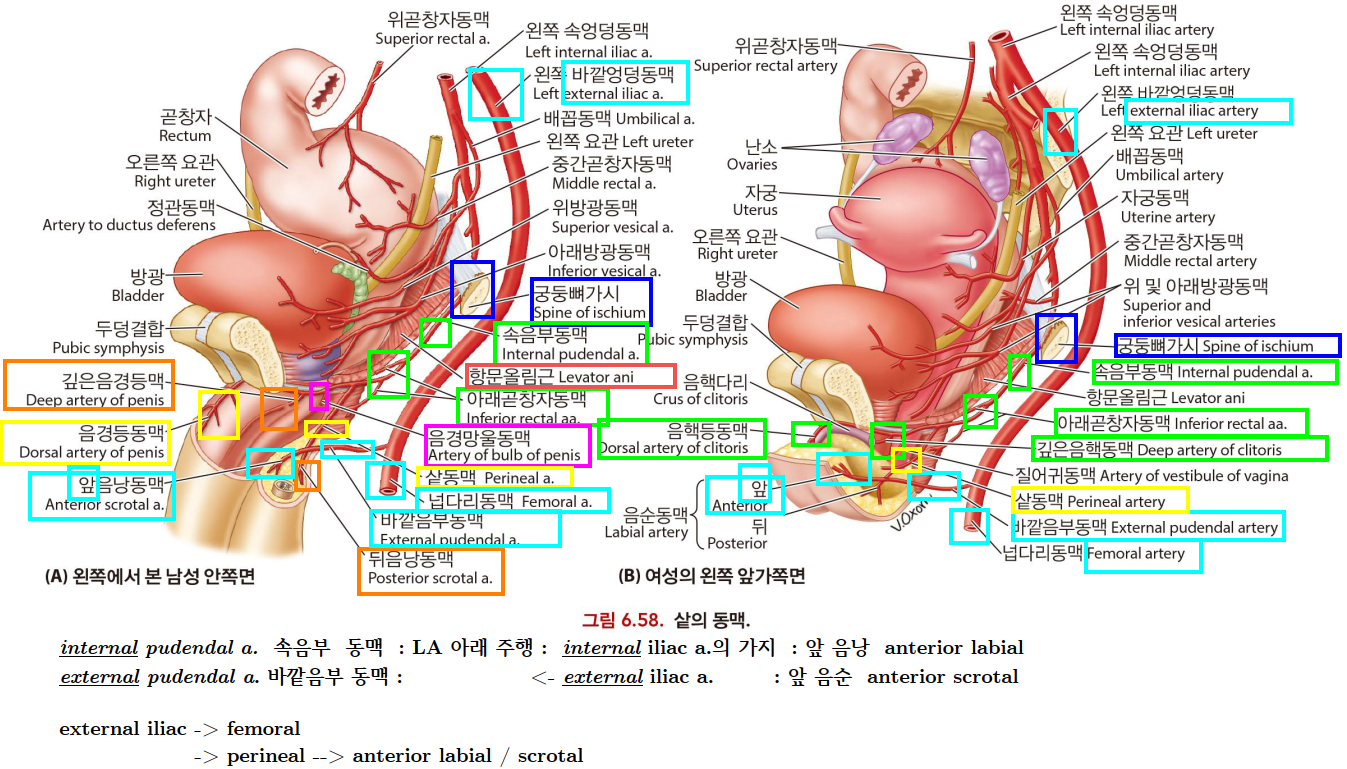
\includegraphics[width=.9\textwidth]{peria.png}
    \label{fig:peria}
\end{figure}
\subsection{샅의 경계}


\begin{enumerate}
\item 위 : 샅의 천장  : 골반가로막 

U자 모양의 비뇨생식틈새 urogenital hiatus ($\subseteq$ 골반가로막) : 요도와 질이 통과 
    \item 두덩결합 
    \item 두덩뼈 
    \item 궁둥뼈 결절 
    \item 엉치결절인대 
    \item 꼬리뼈, 맨마지막 엉치뼈 
\end{enumerate}
\begin{itemize}
    \item 샅막 : 바깥생식기관 부착 , 비뇨생식 구멍 위치 
    
\end{itemize}

\begin{figure}[H]
    \centering
    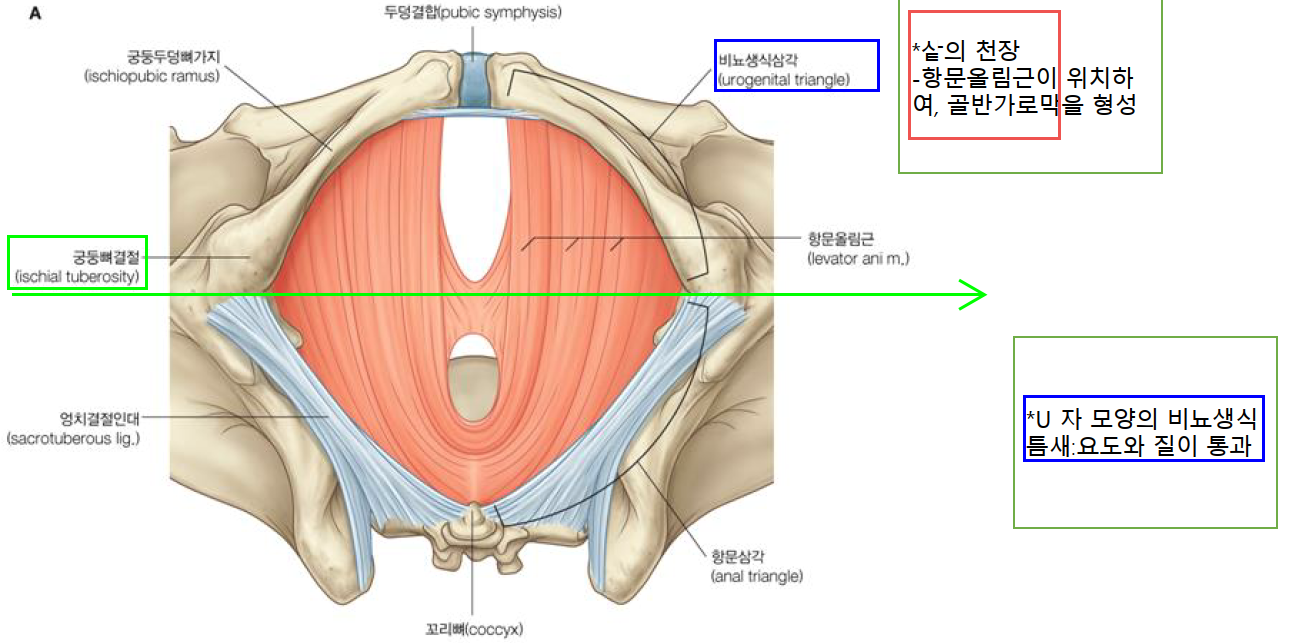
\includegraphics[width=.7\textwidth]{pc1.png}
    \caption{샅의 천장}
    \label{fig:pc1}
\end{figure}

\begin{figure}[H]
    \centering
    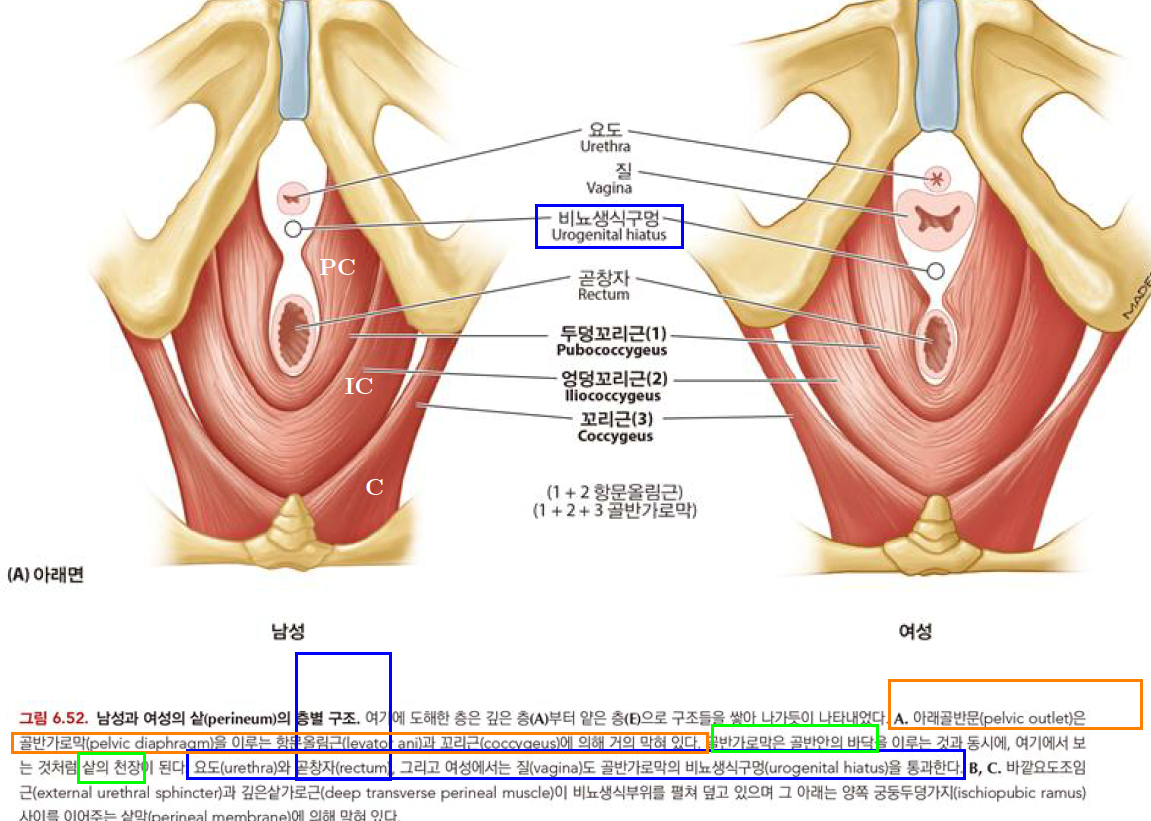
\includegraphics[width=.7\textwidth]{pc2.png}
    \caption{샅의 천장 : 골반가로막}
    \label{fig:pc2}
\end{figure}
\begin{figure}[H]
    \centering
    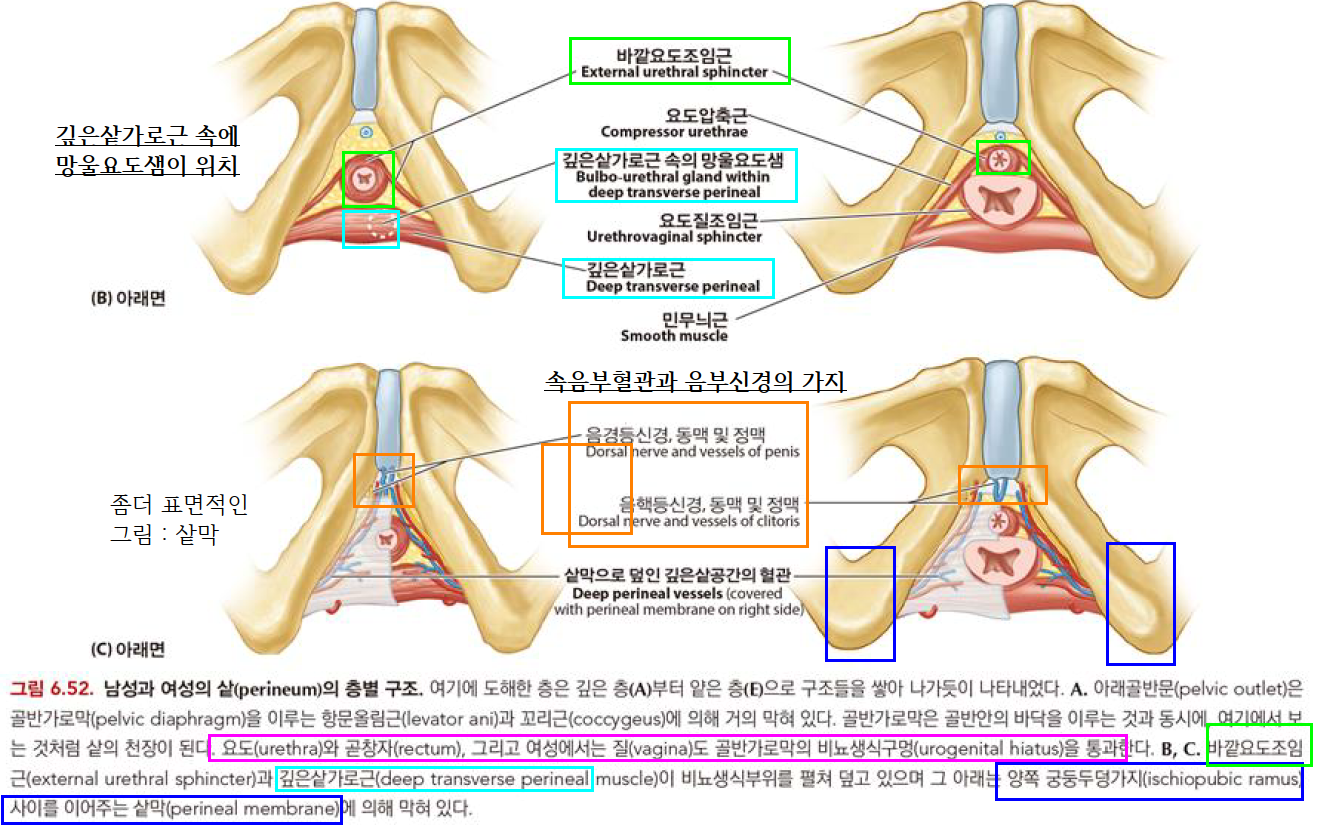
\includegraphics[width=.9\textwidth]{pf1.png}
    \caption{샅의 바닥 : 샅막 }
    \label{fig:pf1}
\end{figure}



\newpage
\subsection{샅의 근막}


골반가로막 

깊은 샅 공간 


샅막 

얕은샅공간 

얕은 샅 근막 


얕은 샅 공간 : 얕은 샅 근막 $\sim $ 샅막


\begin{enumerate}
    \item 얕은샅근막 (피하조직)
    
   
    \begin{enumerate}
        \item 얕은층 (지방층) (fatty fascia)
        
        
         \textbf{대음순}과 \textbf{불두덩(mons pubis)}의 대부분을 구성하며, 남성에서는 지방층이 급격히 줄어
들어, \textbf{음낭근}으로 바뀐다. 남녀 모두에서 \textbf{항문삼각}의 \textbf{궁둥항문오목지방체}와 연속
        \item 깊은층 (막층) (membranous fascia Colles fascia):샅막의 뒤모서리와 샅중심체에 부착되고, 가쪽에서 넙다리근막에 부착되어 항문부
위와 넓적다리로 연속되지 않는다
    \end{enumerate}
    
    \begin{figure}[H]
    \centering
    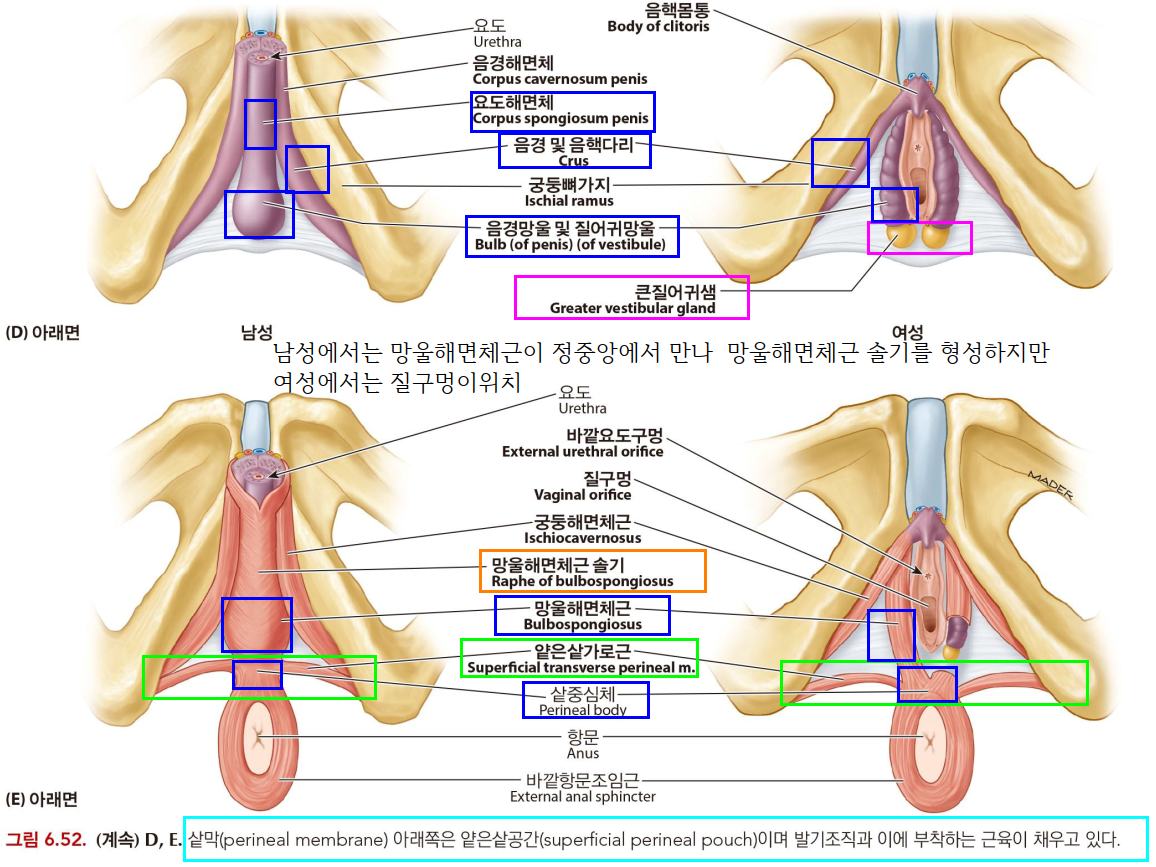
\includegraphics[width=.9\textwidth]{pf2.png}
    \caption{샅막 아래 (얕은 샅 공간)  얕은 샅 근막 위 }
    \label{fig:pf2}
\end{figure}


\begin{figure}[H]
    \centering
    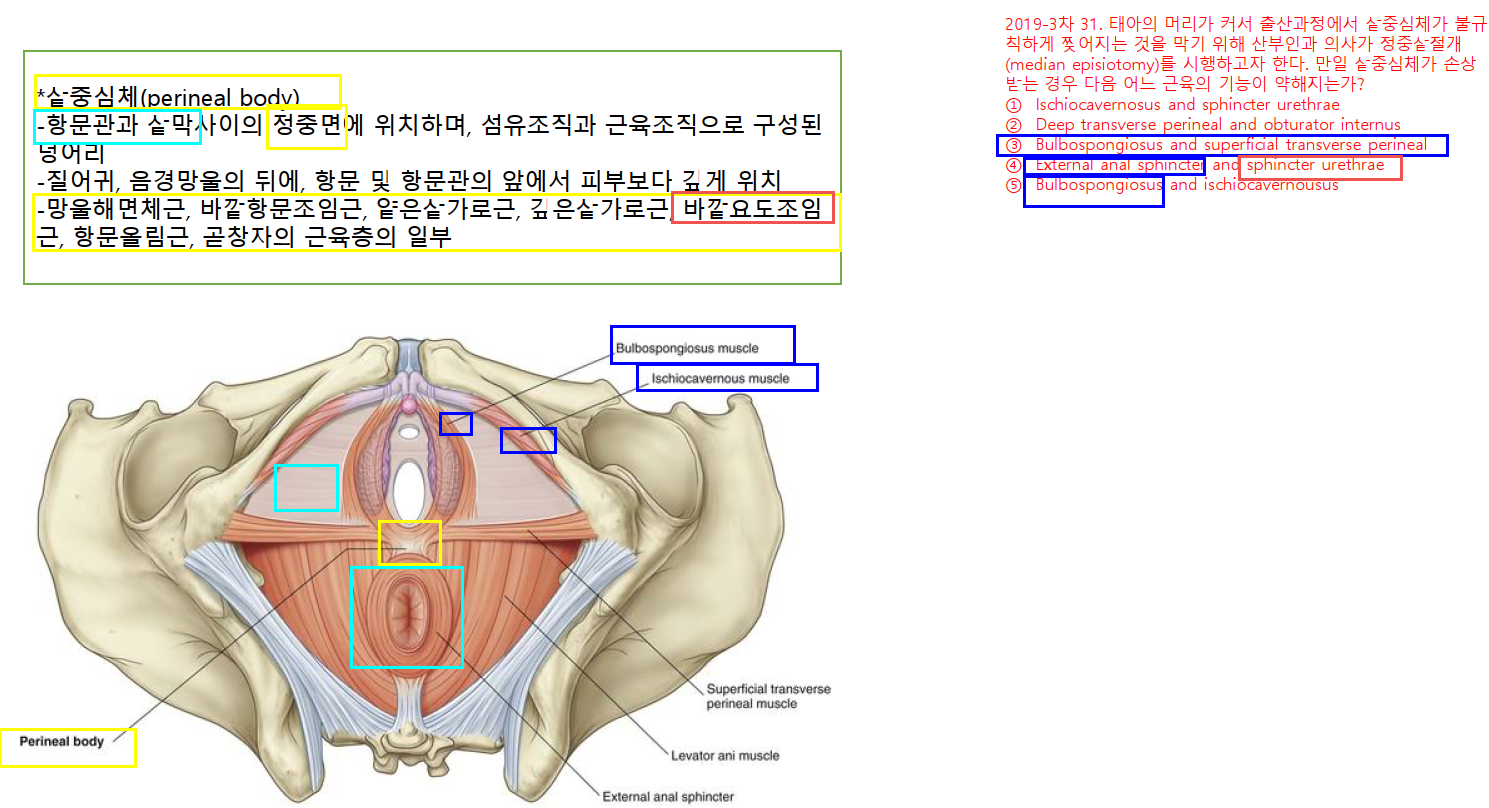
\includegraphics[width=.95\textwidth]{pm1.png}
    \caption{샅막 아래 (얕은 샅 공간) 얕은 샅 근막 위}
    \label{fig:pm1}
\end{figure}

    \begin{figure}[h]
        \centering
        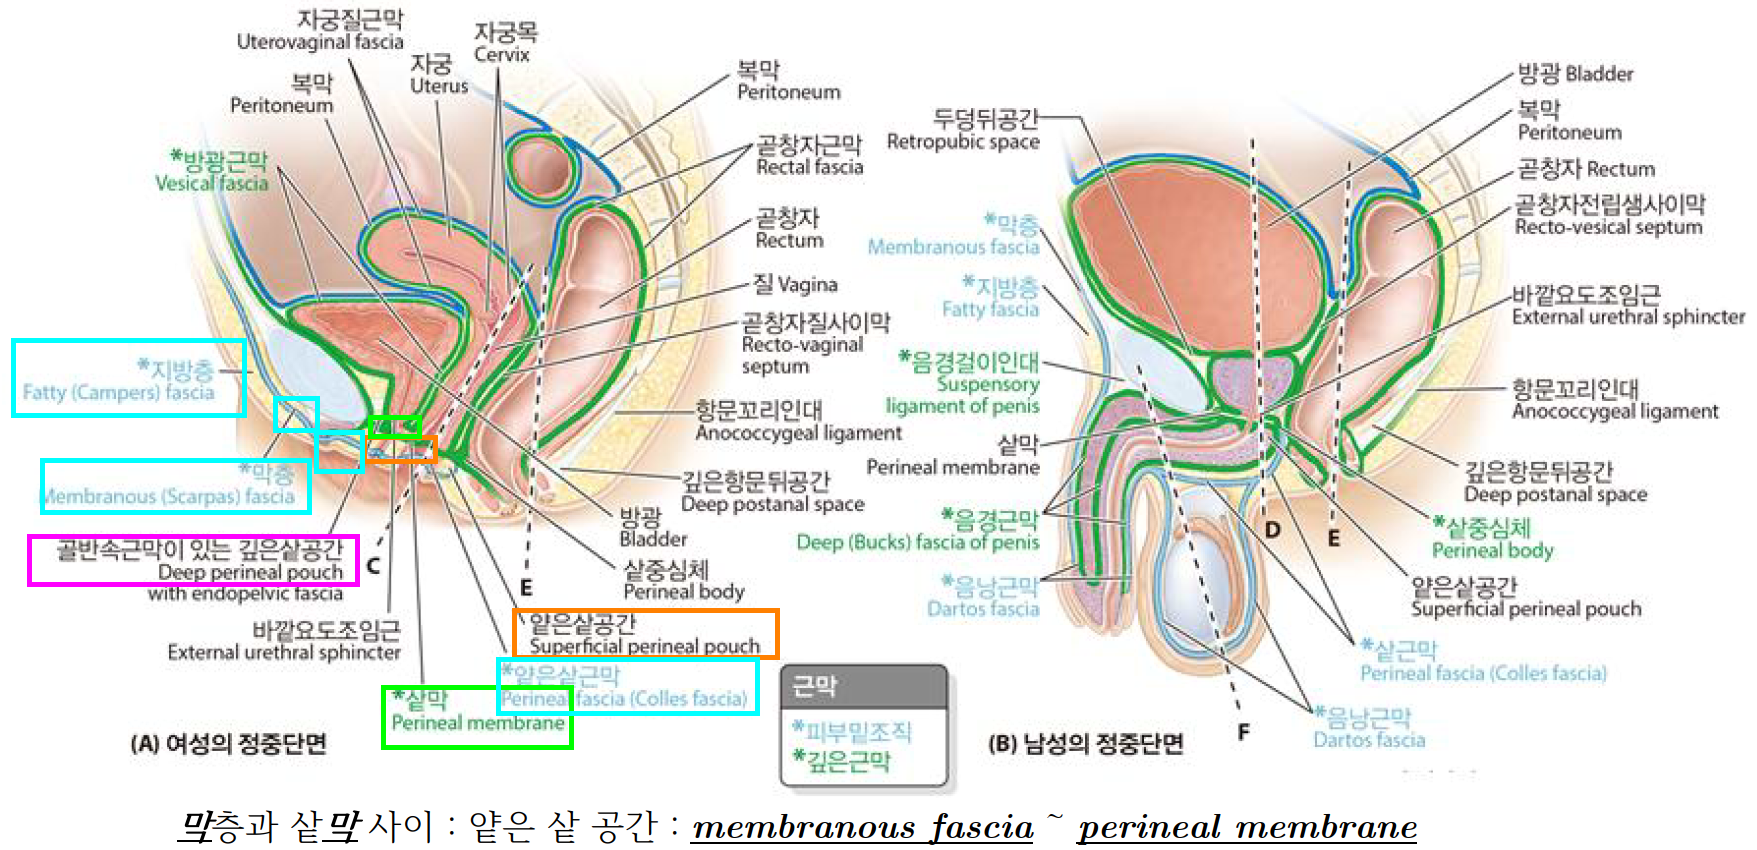
\includegraphics[width=.95\textwidth]{spp.png}
        \caption{superficial perineal pouch : membranous fascia $\sim$ perineal membrane}
        \label{fig:spp}
    \end{figure}
    
    \item 깊은샅근막 
    
    
\end{enumerate}

\subsection{항문삼각과 비뇨생식삼각} 

두 삼각은 동일 평면  X

경계 : 좌우 궁둥뼈가시 사이 가로선 

항문삼각 : 열림 

비뇨생식삼각 : 샅막으로 막힘 
\subsection{}
\section{Rectum}
\subsection{구조}

\begin{table}[H]
    \centering
    \begin{tabular}{c|c|c}
    & above pectinate line & below pectinate line \\ \hline
epithelium    & columnar 원주    & stratified squamous 중층 편평 \\ \hline 
artery     & sra     & mra, ira \\ \hline 
vein & srv $\implies$ imv $\implies$ hepatic portal vein 
& mrv, irv $\implies$ caval venous system \\ \hline
hemorrhoid & internal (not painful) & external (painful) \\ \hline
nerves & inferior hypogastric plexus 아래아랫배신경얼기 &  inferior rectal nerves 아래 곧창자 신경  \\ \hline
lymph &  속엉덩림프절 &  얕은고샅림프절
    \end{tabular}
    \caption{Caption}
    \label{tab:my_label}
\end{table}

\subsubsection{anal canal}

\begin{figure}[H]
    \centering
    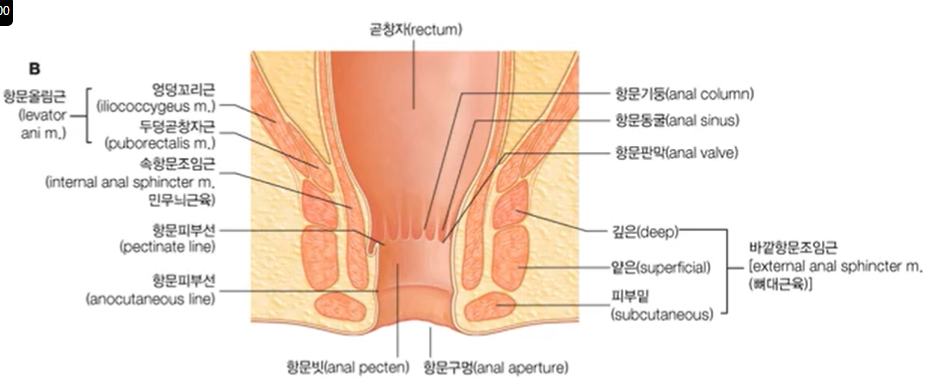
\includegraphics[width=.6\textwidth]{ac1.png}
    \label{fig:ac1}
\end{figure}
\begin{itemize}[label=-]
    \item rectum의 일부 
    (골반가로막의 윗면 - 항문) 
    \item   puborectalis (PR)이 이루는 U자 모양의 걸이 puborectal sling에서 시작하여 뒤 아래쪽으로 내려감 
    \item
    \begin{itemize}  
        \item internal anal sphincter
        
        : 위 2/3 민무늬 불수의근, 창자의 돌림근육이 두꺼워진것 
        
        : 긴장의 원인 : 교감 : 부교감 작용시 수축 억제 
        
        \item 바깥항문조임근 
    \end{itemize}
    \item  anorectal angle 80
    
\end{itemize}

\subsubsection{anal canal의 내부 }
\begin{enumerate}
    \item 항문 기둥 \textbf{column }
    : 위쪽 잘반의 점막에 있는 세로 기둥 
    : sra와 srv의 종말가지가 위치 
    \item 항문곧창자 경계 
: 항문기둥의 위끝 : 곧창자와 항문관의 경계 
\item 
항문판막 \textbf{valve} : 항문기둥의 기둥과 기둥의 아래를 연결하는 초승달모양 주름 
\item 항문굴 : 항문판막 위에 위치한 작은 오목 : 점액을 분비 : 대변을 도움 
\item 빗살선 : 항문판막 아래끝 빗처럼 생긴 선 : 윗부분은 뒤창자에서 유래한 \textbf{내장}부분 : 아래는 항문오목 \textbf{anal pit}에서 유래한 \textbf{ 몸} 부분 
\end{enumerate}

\magenta{구불창자의 \textbf{잘록창자띠}가 곧창자로 가면서 펼쳐져 \textbf{세로근육층}을 형성 }

\begin{figure}[h]
    \centering
    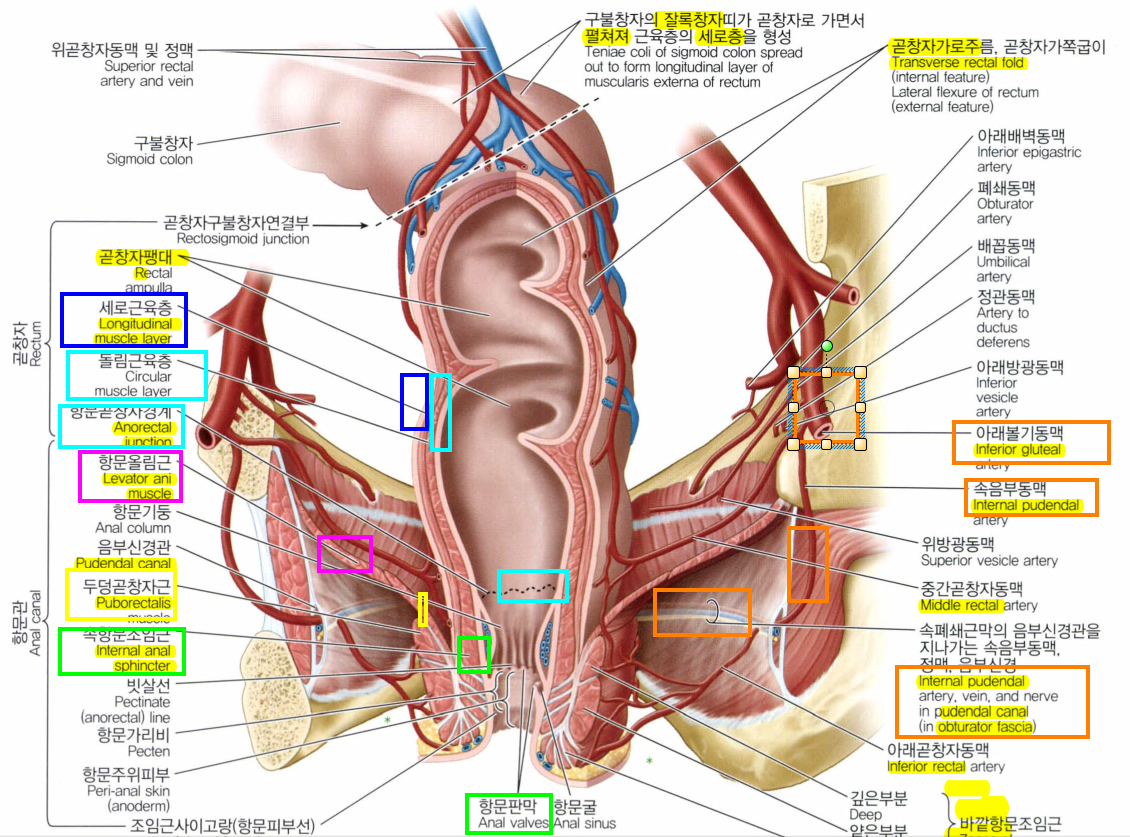
\includegraphics[width=.7\textwidth]{ac2.png}
    \label{fig:ac2}
\end{figure}


\subsection{동맥}
\begin{enumerate}
    \item superior rectum
    $\impliedby$ ima (end branch of inferior mesentric a.)
    \item middle rectum 
$\impliedby $ internal iliac

sra와 ira 연결
\item inferior rectum 

빗살선 아래의 항문관, 항문주위에 분포 
\end{enumerate}

\subsection{정맥 : 속곧창자정맥얼기 }
\begin{enumerate}
    \item 빗살선 위쪽 : srv $\implies$ imv $\implies$ portal vein 
    \item 빗살선 아래 : irv $\implies$ icv 
    \item mrv : srv와 irv 연결 
    
    
\end{enumerate}

\subsection{림프}
\section{Aorta의 가지 }

\vspace{2pt}

\begin{enumerate}

\item  Common Carotid 

\vspace{3pt}

\item Subclavian $\impliedby$ Brachiocephalic trunk 


\begin{enumerate}
    \item \textbf{1st} part 
    
    \begin{enumerate}
        \item vertebral a. 
        \item  internal thoracic
        \begin{itemize}
            \item pericardiaCophrenic  - travels with the phrenic nerve
            
            \item  superior epigastric 
            
            \item    Mediastinal branches
    \item Thymic branches
    \item  Sternal branches
\item Perforating branches

\item  
Twelve \textit{\textbf{anterior intercostal}} branches, two to each of the \textit{\textbf{top six intercostal}}  spaces.


 In a given space, the upper branch travels laterally along the bottom of the rib until it \textbf{anastomoses} with its corresponding \textbf{posterior intercostal} artery. The lower branch of the space anastomoses with a collateral branch of the posterior intercostal artery.
After passing the sixth intercostal space, the internal thoracic artery splits into the following \textit{\textbf{two}} \textbf{terminal branches} :

\textit{\textbf{Musculophrenic}}  artery - roughly follows the costal margin


\textit{\textbf{Superior epigastric}} artery - continues the course of the internal thoracic artery, travelling downward into the abdominal wall
        \end{itemize}
        \item thyrocervical 
    \end{enumerate}
    
    \item \textbf{2nd} part 
 :     costocervical trunk
    \begin{enumerate}
        \item deep cervical 
        
        \item highest intercostal 
    \end{enumerate}
    
    \item \textbf{3rd} part 
    
    \begin{enumerate}
        \item dorsal scapular 
    \end{enumerate}
\end{enumerate}


\vspace{3pt}


\item  Axillary 



\vspace{3pt}

\item Descending Thoracic Aorta (뒤세로칸 posterior mediastium)

\vspace{3pt}

\begin{enumerate}
    \item 
    superior phrenic a. 
    
\end{enumerate}

\vspace{3pt}

\item Abdominal aorta


abdominal : diaphragm 밑  $\implies $ 1st 가지가 inferior phrenic


\begin{enumerate}
\item inferior phrenic (T12)

\vspace{1.5pt}

\item  celiac (T12)


\vspace{1.5pt}

\item  Superior Mesenteric (L1)

\item Suprarenal (superior, middle (L1), inferior) 
\begin{enumerate}
    \item superior suprarenal ($\impliedby$ inferior phrenic)
    \item middle superarenal ($\impliedby$ abdominal aorta)
    
    middle : 그냥중간 : 가지가 아니라 그냥 aorta
    \item inferior suprarenal ($\impliedby $ renal a.)
    
    (inferior랑 supra 상쇄해서 없어져서 그냥 renal 됨) 
    
    
\end{enumerate}

    \vspace{1.5pt}
    
    
    \item 
    
    Renal artery (LV 1$\sim$2) disc
    
    \vspace{1.5pt}
    
    
    \item Inferior phrenic  (T12-L2 : variety in origin)
    
\item   Gonadal (L2) 

\item  Lumbar (L1-L4)

\item inferior mesenteric (L3)

\item  median sacral (L4)

\item common iliac (L4) 
    \end{enumerate}
\end{enumerate}

\vspace{2pt}




%-------------------------------------------------------------------------
\newpage
\begin{prob}{1}
\textnormal{요관 결석증이 가장 빈번하게 생기는 부위는 어디입니까?}

\end{prob}

\begin{solution}

\textcolor{white}{124}

\begin{enumerate}
    \item 콩팥깔때기와 요관의 연결부위
    \item 요관이 바깥엉덩동맥과 골반 가장자리를 건너가는 부위
    \item 요관이 방광벽을 통과하는 부위
    
\end{enumerate}

가 자연적으로 좁은 부위라서 요관 결석이 가장 빈번하게 생깁니다.
\end{solution}


\textcolor{white}{124} \\

\begin{prob}{2}
\textnormal{
남성 요도의 근육 중에서 여성 요도에서는 필요하지 않은 근육이 무엇입니까?}
\end{prob}
\begin{solution}
 여성요도는 
생식계통과 연결되어 있지 않으므로 여성에서는 방굉목에 속요도조임근 
(internal urethral sphincter)이 필요하지 않습니다.

\end{solution}
\section{Rectum}
\begin{prob}{3}
\textnormal{곧창자벽을 통해 곧창자의 앞아래에 있는 어떤  구조를 촉진할 수 있습니까?}
\end{prob}
\begin{solution}
남성의 전립샘과 정액샘, 여성의 자궁목을 촉진할 수 있습니디ㅏ. 남성과 여성 모두 영치 뼈 골반면과 꼬리뼈를 촉진 할 수 있습니다.  궁퉁뼈가시와 궁퉁뼈결절이 만져질 때도 있습니다. 부어오른 속 
영덩림프절과 요관의 병적인 비 후(pathological thickening), 그리고 궁둥항문오목고름집 (ischioanal abscess, 416 쪽)과 남성의 곧창자방광오목이나 여성의 곧창자자궁오목에 비정상적인 덩어리가 있다든지 하여 나타나는 궁둥항문오목의 종쟁(swelling) 도 촉진이 기능하다. 염증이 생긴 막창자꼬리 (appendix) 가 작은골반, 특히 곧창자옆오목으로 내려오게  되면 곧창자검사를 통해 압됨(tendemess) 이 느껴질 수 있습니다.

\end{solution}

\end{document}
